% answers.tex —— 1977 年·江苏苏州地区初试卷 · 参考答案与详细解析片段
% 由 tools/generate_projects.py 依来源总账自 1977/1977_数学真题_江苏苏州地区初试_试题.md + 1977/1977_数学真题_江苏苏州地区初试_解析正文.md + 1977/1977_数学真题_江苏苏州地区初试_答案要点.md 生成，勿手改（改源 MD 后重跑）


\begin{gktip}
固定源为两页纯题面扫描（原书页码 248 起），未附解答。下文各题由编者独立推导。原卷大题号「一、二、三、四、五、六」已转写为阿拉伯数字；大题一、二、三的小题「1．2．…」与大题五已有的「（1）（2）（3）」统一为「（N）」，未增删题干。原卷末尾「附加题」两题按本库规范排在最后一题解析之后。
\end{gktip}

\begin{answer}
\gksolhead{1}{}

\textbf{题目}：

（1） 化简：$(3y-1)^2-(3y-1)(3y+1)+3(y-1)$。

（2） 因式分解：$4x^4-y^4$。

（3） 计算：$(a+b-c)(a-b+c)$。

\Needspace{5\baselineskip}
（4） 计算：

\nopagebreak[4]
\[
\left(\frac{a-2b}{a+2b}-\frac{a+2b}{a-2b}\right)\div\frac{4ab}{4b^2c-a^2c}.
\]

\Needspace{5\baselineskip}
（5） 计算：

\nopagebreak[4]
\[
\sqrt[3]{1-\sqrt2}\cdot\sqrt[6]{3+2\sqrt2}-\frac1{1-\sqrt2}.
\]

\Needspace{4\baselineskip}
\textbf{解析}

\gksubpart{（1）}

\nopagebreak[4]
\[
\begin{aligned}
(3y-1)^2-(3y-1)(3y+1)+3(y-1)
&=(9y^2-6y+1)-(9y^2-1)+(3y-3)\\
&=-6y+1+1+3y-3\\
&=-3y-1.
\end{aligned}
\]

\gksubpart{（2）}

\nopagebreak[4]
\[
4x^4-y^4=(2x^2-y^2)(2x^2+y^2).
\]

\gksubpart{（3）}

\nopagebreak[4]
\[
(a+b-c)(a-b+c)=a^2-(b-c)^2=a^2-b^2-c^2+2bc.
\]

\gksubpart{（4）}

\Needspace{5\baselineskip}
设 $p=a+2b$，$q=a-2b$，则

\nopagebreak[4]
\[
\frac{q}{p}-\frac{p}{q}=\frac{q^2-p^2}{pq}
=\frac{(a-2b)^2-(a+2b)^2}{(a+2b)(a-2b)}
=\frac{-8ab}{a^2-4b^2}.
\]

\Needspace{5\baselineskip}
又 $4b^2c-a^2c=-c(a^2-4b^2)$，故

\nopagebreak[4]
\[
\left(\frac{a-2b}{a+2b}-\frac{a+2b}{a-2b}\right)\div\frac{4ab}{4b^2c-a^2c}
=\frac{-8ab}{a^2-4b^2}\times\frac{-c(a^2-4b^2)}{4ab}
=2c.
\]

\gksubpart{（5）}

\Needspace{5\baselineskip}
注意到 $3+2\sqrt2=(\sqrt2+1)^2$，故

\nopagebreak[4]
\[
\sqrt[6]{3+2\sqrt2}=\sqrt[6]{(\sqrt2+1)^2}=\sqrt[3]{\sqrt2+1}.
\]

\Needspace{5\baselineskip}
于是

\nopagebreak[4]
\[
\sqrt[3]{1-\sqrt2}\cdot\sqrt[6]{3+2\sqrt2}
=\sqrt[3]{(1-\sqrt2)(1+\sqrt2)}
=\sqrt[3]{-1}=-1.
\]

\Needspace{5\baselineskip}
又

\nopagebreak[4]
\[
\frac1{1-\sqrt2}=\frac{1+\sqrt2}{(1-\sqrt2)(1+\sqrt2)}=\frac{1+\sqrt2}{-1}=-(1+\sqrt2).
\]

\Needspace{5\baselineskip}
所以原式

\nopagebreak[4]
\[
=-1-\bigl[-(1+\sqrt2)\bigr]=-1+1+\sqrt2=\sqrt2.
\]

\gkanswer{答案（1）：$-3y-1$。}

\gkanswer{答案（2）：$(2x^2-y^2)(2x^2+y^2)$。}

\gkanswer{答案（3）：$a^2-b^2-c^2+2bc$。}

\gkanswer{答案（4）：$2c$。}

\gkanswer{答案（5）：$\sqrt2$。}

\end{answer}
\begin{answer}
\gksolhead{2}{}

\textbf{题目}：

\Needspace{5\baselineskip}
（1） 解方程：

\nopagebreak[4]
\[
3+\frac{5x-1}{2}=x-\frac{1-3x}{5}.
\]

（2） 解方程：$x^2+x-2=0$。

\Needspace{5\baselineskip}
（3） 解方程组：

\nopagebreak[4]
\[
\begin{cases}
3x+2y-1=0\\
2x-3y+8=0
\end{cases}
\]

（4） 解不等式：$3(2y-5)+4\geqslant8y-7$。

\Needspace{4\baselineskip}
\textbf{解析}

\gksubpart{（1）}

\Needspace{5\baselineskip}
两边乘以 $10$（$2$ 与 $5$ 的最小公倍数）：

\nopagebreak[4]
\[
30+5(5x-1)=10x-2(1-3x).
\]

\Needspace{5\baselineskip}
展开：$30+25x-5=10x-2+6x$，即 $25x+25=16x-2$，解得

\nopagebreak[4]
\[
9x=-27,\qquad x=-3.
\]

\gksubpart{（2）}

\nopagebreak[4]
\[
x^2+x-2=0\quad\Longrightarrow\quad(x+2)(x-1)=0,
\]

故 $x=-2$ 或 $x=1$。

\gksubpart{（3）}

\nopagebreak[4]
\[
\begin{cases}
3x+2y-1=0\\
2x-3y+8=0
\end{cases}
\]

\Needspace{5\baselineskip}
第一式乘 $3$、第二式乘 $2$ 后相加消去 $y$：

\nopagebreak[4]
\[
9x+6y=3,\qquad 4x-6y=-16,
\]

相加得 $13x=-13$，即 $x=-1$。代回第一式：$-3+2y=1$，得 $y=2$。

\gksubpart{（4）}

\nopagebreak[4]
\[
3(2y-5)+4\geqslant8y-7
\quad\Longrightarrow\quad
6y-11\geqslant8y-7
\quad\Longrightarrow\quad
-4\geqslant2y,
\]

故 $y\leqslant-2$。

\gkanswer{答案（1）：$x=-3$。}

\gkanswer{答案（2）：$x=1$ 或 $x=-2$。}

\gkanswer{答案（3）：$x=-1$，$y=2$。}

\gkanswer{答案（4）：$y\leqslant-2$。}

\end{answer}
\begin{answer}
\gksolhead{3}{}

\textbf{题目}：

（1） 计算：$4\sin30^\circ-3\operatorname{tg}45^\circ+2\cos30^\circ$。

（2） 在 $\triangle ABC$ 中，$C=90^\circ$，$a=2$，$b=1$，求 $\sin B$，$\operatorname{tg}A$。

（3） 在 $\triangle ABC$ 中，$M\text{、}N$ 分别是 $AB\text{、}AC$ 的中点，如果 $\triangle ABC$ 的面积是 $20$ 平方厘米，求 $\triangle AMN$ 的面积。

（4） 如图，$AB$ 为半圆的直径，$CD\perp AB$，求证：$CD^2=AD\cdot BD$。

\begin{gktip}
原源 PDF 第 1 页附有半圆、直径与垂线的示意图；LaTeX 版按源图重绘。
\end{gktip}
\nopagebreak[4]
\begin{center}% 1977 年江苏苏州地区初试卷第三题（4）小题：AB 为半圆的直径，CD⊥AB 于 D，C 在圆上（按源卷第1页布局）
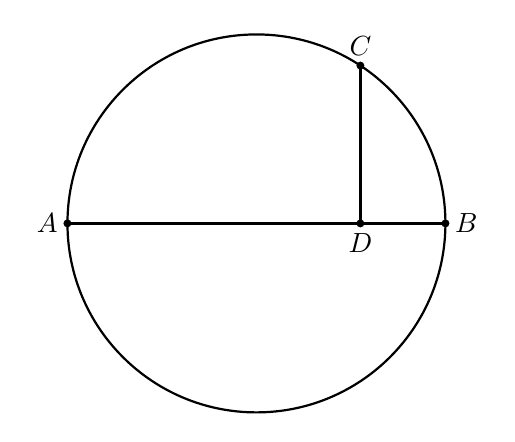
\begin{tikzpicture}[scale=1.2]
  \coordinate (O) at (0,0);
  \coordinate (A) at (-2,0);
  \coordinate (B) at (2,0);
  \coordinate (D) at (1.1,0);
  \coordinate (C) at (1.1,1.67);
  \draw[thick] (O) circle (2);
  \draw[thick] (A)--(B);
  \draw[thick] (C)--(D);
  \fill (A) circle (1.2pt) node[left] {$A$};
  \fill (B) circle (1.2pt) node[right] {$B$};
  \fill (C) circle (1.2pt) node[above] {$C$};
  \fill (D) circle (1.2pt) node[below] {$D$};
\end{tikzpicture}
\end{center}
\nopagebreak[4]
（5） 求 $P_1(0,-5)$ 和 $P_2(-1,2)$ 两点间的距离。

\Needspace{4\baselineskip}
\textbf{解析}

\gksubpart{（1）}

\nopagebreak[4]
\[
4\sin30^\circ-3\operatorname{tg}45^\circ+2\cos30^\circ
=4\times\frac12-3\times1+2\times\frac{\sqrt3}2
=2-3+\sqrt3=\sqrt3-1.
\]

\gksubpart{（2）}

\Needspace{5\baselineskip}
$C=90^\circ$，故 $c=\sqrt{a^2+b^2}=\sqrt{4+1}=\sqrt5$。因此

\nopagebreak[4]
\[
\sin B=\frac bc=\frac1{\sqrt5}=\frac{\sqrt5}5,
\qquad
\operatorname{tg}A=\frac ab=\frac21=2.
\]

\gksubpart{（3）}

\Needspace{5\baselineskip}
$M\text{、}N$ 分别是 $AB\text{、}AC$ 的中点，故 $\triangle AMN\sim\triangle ABC$，相似比为 $\dfrac12$，面积比为 $\dfrac14$。所以

\nopagebreak[4]
\[
S_{\triangle AMN}=20\times\frac14=5\ (\text{\text{平方厘米}}).
\]

\gksubpart{（4）}

\Needspace{5\baselineskip}
$AB$ 为半圆的直径，故 $\angle ACB=90^\circ$（直径所对的圆周角）。在 $\mathrm{Rt}\triangle ACB$ 中，$CD$ 是斜边 $AB$ 上的高，$\triangle ADC\sim\triangle CDB$（两者都是直角三角形，且 $\angle DAC=\angle DCB$，因为它们都与 $\angle ACD$ 互余）。由相似得

\nopagebreak[4]
\[
\frac{AD}{CD}=\frac{CD}{BD}
\quad\Longrightarrow\quad
CD^2=AD\cdot BD.
\]
\nopagebreak[4]
\begin{center}% 1977 年江苏苏州地区初试卷第三题（4）小题：AB 为半圆的直径，CD⊥AB 于 D，C 在圆上（按源卷第1页布局）
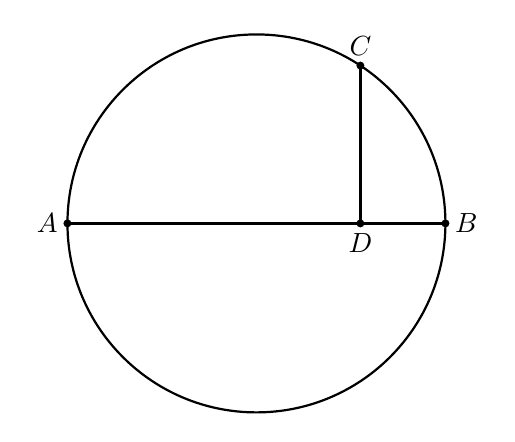
\begin{tikzpicture}[scale=1.2]
  \coordinate (O) at (0,0);
  \coordinate (A) at (-2,0);
  \coordinate (B) at (2,0);
  \coordinate (D) at (1.1,0);
  \coordinate (C) at (1.1,1.67);
  \draw[thick] (O) circle (2);
  \draw[thick] (A)--(B);
  \draw[thick] (C)--(D);
  \fill (A) circle (1.2pt) node[left] {$A$};
  \fill (B) circle (1.2pt) node[right] {$B$};
  \fill (C) circle (1.2pt) node[above] {$C$};
  \fill (D) circle (1.2pt) node[below] {$D$};
\end{tikzpicture}
\end{center}
\nopagebreak[4]
\gksubpart{（5）}

\nopagebreak[4]
\[
|P_1P_2|=\sqrt{(0-(-1))^2+(-5-2)^2}=\sqrt{1+49}=\sqrt{50}=5\sqrt2.
\]

\gkanswer{答案（1）：$\sqrt3-1$。}

\gkanswer{答案（2）：$\sin B=\dfrac{\sqrt5}{5}$，$\operatorname{tg}A=2$。}

\gkanswer{答案（3）：$5$ 平方厘米。}

\gkanswer{答案（4）：见解析版}

\gkanswer{答案（5）：$5\sqrt2$。}

\end{answer}
\begin{answer}
\gksolhead{4}{}

\textbf{题目}：

某机器厂第三季度共制造机器 $331$ 台，已知七月份制造 $100$ 台，求第三季度的月平均增长率。

\Needspace{4\baselineskip}
\textbf{解析}

\Needspace{5\baselineskip}
设月平均增长率为 $x$，七月份产量为 $100$ 台，八、九月份产量分别为 $100(1+x)$、$100(1+x)^2$。由第三季度共制造 $331$ 台，

\nopagebreak[4]
\[
100\bigl[1+(1+x)+(1+x)^2\bigr]=331.
\]

\Needspace{5\baselineskip}
令 $t=1+x$，则

\nopagebreak[4]
\[
t^2+t+1=3.31\quad\Longrightarrow\quad t^2+t-2.31=0.
\]

\Needspace{5\baselineskip}
解得

\nopagebreak[4]
\[
t=\frac{-1\pm\sqrt{1+9.24}}2=\frac{-1\pm3.2}2,
\]

取正值 $t=1.1$（$t=-2.1$ 不合题意，舍去），故 $x=t-1=0.1$，即月平均增长率为 $10\%$。

\gkanswer{答案：月平均增长率为 $10\%$。}

\end{answer}
\begin{answer}
\gksolhead{5}{}

\textbf{题目}：

在 $\triangle ABC$ 中，$A=45^\circ$，$AB+AC=10\ \mathrm{cm}$，

（1） 用公式法表示 $\triangle ABC$ 的面积 $(S)$ 与一边长 $AB\ (x)$ 之间的函数关系；

（2） $x$ 为何值时 $S$ 为最大；

（3） 求 $S$ 的最大值。

\Needspace{4\baselineskip}
\textbf{解析}

\gksubpart{（1）}

\Needspace{5\baselineskip}
设 $AB=x$，则 $AC=10-x$（$0<x<10$）。由面积公式

\nopagebreak[4]
\[
S=\frac12\cdot AB\cdot AC\cdot\sin A
=\frac12x(10-x)\sin45^\circ
=\frac{\sqrt2}4x(10-x)\qquad(0<x<10).
\]

\gksubpart{（2）}

\nopagebreak[4]
\[
S=\frac{\sqrt2}4(10x-x^2)=-\frac{\sqrt2}4(x-5)^2+\frac{25\sqrt2}4,
\]

在 $(0,10)$ 内，$x=5$ 时 $S$ 取最大值。

\gksubpart{（3）}

\nopagebreak[4]
\[
S_{\max}=\frac{25\sqrt2}4\ (\text{\text{平方厘米}}).
\]

\gkanswer{答案（1）：$S=\dfrac{\sqrt2}{4}x(10-x)$（$0<x<10$）。}

\gkanswer{答案（2）：$x=5$（$\mathrm{cm}$）时 $S$ 最大。}

\gkanswer{答案（3）：$S$ 的最大值为 $\dfrac{25\sqrt2}{4}$ 平方厘米。}

\end{answer}
\begin{answer}
\gksolhead{6}{}

\textbf{题目}：

过点 $P(1,0)$ 作圆 $(x+1)^2+y^2=1$ 的切线，求切线方程。

\textbf{附加题 1．} 求所有被 $3$ 除余数为 $1$ 的两位数的和。

\textbf{附加题 2．} 求立方抛物线 $y=x^3$ 和直线 $y=1$、$x=0$ 所围成的图形的面积。

\begin{gktip}
提示：$1^3+2^3+3^3+\cdots+n^3=\left[\dfrac{n(n+1)}{2}\right]^2$。
\end{gktip}

\Needspace{4\baselineskip}
\textbf{解析}

\Needspace{5\baselineskip}
圆心为 $(-1,0)$，半径 $r=1$。$P(1,0)$ 到圆心的距离为 $2>r$，故 $P$ 在圆外；直线 $x=1$ 到圆心的距离为 $2\ne1$，非切线，故设切线为 $y=k(x-1)$，即 $kx-y-k=0$。圆心到该直线的距离为

\nopagebreak[4]
\[
d=\frac{|k(-1)-0-k|}{\sqrt{k^2+1}}=\frac{2|k|}{\sqrt{k^2+1}}.
\]

\Needspace{5\baselineskip}
令 $d=1$：

\nopagebreak[4]
\[
4k^2=k^2+1\quad\Longrightarrow\quad k^2=\frac13\quad\Longrightarrow\quad k=\pm\frac{\sqrt3}3.
\]

\Needspace{5\baselineskip}
代入并整理，得两条切线方程：

\nopagebreak[4]
\[
x-\sqrt3y-1=0,\qquad x+\sqrt3y-1=0.
\]

\textbf{附加题 1}

\Needspace{5\baselineskip}
被 $3$ 除余 $1$ 的两位数是首项 $10$、末项 $97$、公差 $3$ 的等差数列，项数

\nopagebreak[4]
\[
n=\frac{97-10}3+1=30.
\]

\Needspace{5\baselineskip}
其和为

\nopagebreak[4]
\[
S=\frac{n(10+97)}2=\frac{30\times107}2=1605.
\]

\textbf{附加题 2}

\Needspace{5\baselineskip}
先求 $\displaystyle\int_0^1x^3\,dx$。把 $[0,1]$ 分成 $n$ 等份，取右端点 $x_i=\dfrac in$，则

\nopagebreak[4]
\[
\sum_{i=1}^n x_i^3\cdot\frac1n=\frac1{n^4}\sum_{i=1}^ni^3
=\frac1{n^4}\left[\frac{n(n+1)}2\right]^2
=\frac{(n+1)^2}{4n^2}.
\]

\Needspace{5\baselineskip}
令 $n\to\infty$，得

\nopagebreak[4]
\[
\int_0^1x^3\,dx=\lim_{n\to\infty}\frac{(n+1)^2}{4n^2}=\frac14.
\]

\Needspace{5\baselineskip}
因此曲线 $y=x^3$、直线 $y=1$、$x=0$ 所围成的图形面积为

\nopagebreak[4]
\[
S=1\times1-\int_0^1x^3\,dx=1-\frac14=\frac34.
\]

\gkanswer{答案：切线方程为 $x-\sqrt3y-1=0$ 和 $x+\sqrt3y-1=0$。}

\end{answer}